\section{Metoda skokowa}
%%%%%%%%%%%%%%%%%%%%%
\begin{frame}{Metoda skokowa}
	\begin{block}{Założenia}
	\begin{itemize}
	\item pochodną względem czasu określamy na podwójnym kroku
    \item kroku pośredniego używamy dla określenia całki
    \item metoda wycentrowana w czasie $\rightarrow $ dokładność drugiego rzędu $\varepsilon = 0({\Delta t}^2)$
	\end{itemize}
	\end{block}
\end{frame}
%%%%%%%%%%%%%%%%%%%%%
\begin{frame}{Algorytm}
	\begin{figure}
	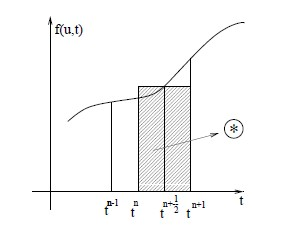
\includegraphics[height=0.5\textheight]{img/22/metoda_skokowa.jpg}
	\end{figure}
    \textbf{Algorytm:}
    $$ \begin{array}{rcl}
      (n+1):\quad &=&u^{n-1} -f(u^n,t^n)\cdot 2 \cdot \Delta t\\
      (n+2):\quad &=&u^n \quad -f(u^{n+1},t^{n+1})\cdot 2 \cdot \Delta t
      \end{array} $$
    
\end{frame}
%%%%%%%%%%%%%%%%%%%%%

\begin{frame}{Trudności}
	\begin{enumerate}
      \item znamy $u^0 = u(0)$, potrzebne $u^1 = u(\Delta t)$; od $u^1$ zależy całkowita dokładność
          \begin{itemize}
            \item podprzedziały w pierwszym $\Delta t$, metoda Eulera,
            \item rozwinięcie w szereg wyższych potęg,
          \end{itemize}
      \item zagadnienie nieliniowe $\Rightarrow$ zmienne $\Delta t$ \quad metoda przestaje być wycentrowana w czasie
    \end{enumerate}
\end{frame}
%%%%%%%%%%%%%%%%%%%%%
\begin{frame}{Współczynnik wzmocnienia błędu}
	$$\varepsilon^{n+1} = \varepsilon^{n-1} - \frac{\partial f}{\partial u} \bigg\arrowvert _n \cdot 2 \cdot \Delta t \cdot \varepsilon^n \quad \arrowvert :\varepsilon^{n-1}$$
    $$\alpha = \frac{\partial f}{\partial u}\bigg\arrowvert_n \cdot \Delta t \qquad g = \frac{\varepsilon^{n+1}}{\varepsilon^n} \ldots$$
    $$g^2 = 1- \alpha \cdot 2g \qquad \underline{g = -\alpha \pm \sqrt{\alpha^2+1}}$$
    Dla metod drugiego rzędu zawsze mamy dwa pierwiastki. \newline
    $\alpha$ - rzeczywiste $\Rightarrow$ \quad $|g| > 1$ \quad $\rightarrow$ niestabilna \quad $\alpha = i\beta, \beta \leqslant 1$, rzeczywiste \newline
    $\Rightarrow g = -i\beta\pm\sqrt{1-\beta^2} \qquad |g|^2 = g \cdot g^* = 1 \quad dla \quad \frac{du}{dt}+i\omega u = 0 \rightarrow \quad \beta = \omega\Delta t \leqslant 1 \quad \rightarrow \quad \Delta t \leqslant\frac{1}{\omega}$
\end{frame}
\begin{frame}{Metoda skokowa dla równań rozpadu}
	$$\frac{du}{dt}+\underbrace{\frac{u}{\tau}}_{f(u,t)} = 0$$\par
    $$ \begin{array}{rcl}
      (n+1):\quad &=&u^{n-1} -f(u^n,t^n)\cdot 2 \cdot \Delta t\\
      (n+2):\quad &=&u^n \quad -f(u^{n+1},t^{n+1})\cdot 2 \cdot \Delta t
      \end{array} $$
      $$\left\{\begin{array}{lll}
      \text{siatka parzysta:}& \text{węzły } 2n&\text{zmienna } \eta\\
      \text{siatka nieparzysta:}&\text{węzły } 2n+1& \text{zmienna }\chi
      \end{array}\right\}\text{  słabo związane}$$
      $$\left\{\begin{array}{lcl}
      \eta^{2n} &=& \eta^{2n-1} - \chi^{2n-1} \cdot\frac{2\Delta t}{\tau}\\
      \chi^{2n+1} &=& \chi^{2n-1} - \eta^{2n} \cdot\frac{2\Delta t}{\tau}
    \end{array}\right.$$
\end{frame}
%%%%%%%%%%%%%%%%%%%%%
\begin{frame}
	Te równania różnicowe są równoważne :
    $$\left\{\begin{array}{lcl}
      \frac{d\eta}{dt}+\frac{\chi}{\tau}&=&0\\
      \frac{d\chi}{dt}+\frac{\eta}{\tau}&=&0
    \end{array}\right.$$
    Dodanie i odjęcie powyższych równań $\Rightarrow$ \quad \textbf{stany własne układu}
    $$\left\{\begin{array}{lcl}
      \frac{d}{dt}(\eta+\chi)+\frac{\eta+\chi}{\tau} & = & 0 \quad \Rightarrow \text{składowa, której szukamy }\\
       & & \qquad \text{(spełnia równanie wyjściowe)}\\
      \frac{d}{dt}(\eta-\chi)+\frac{\eta-\chi}{\tau} & = & 0 \quad \Rightarrow \text{składowa numeryczna,} \\
      & & \qquad \text{zależy od dokładności } u^1\\
      & & \qquad \text{nie jest zgodna z równaniem wyjściowym}
    \end{array}\right.$$
\end{frame}
%%%%%%%%%%%%%%%%%%%%%%%%%%v
